%                                                                 aa.dem
% AA vers. 8.2, LaTeX class for Astronomy & Astrophysics
% demonstration file
%                                                       (c) EDP Sciences
%-----------------------------------------------------------------------
%
%\documentclass[referee]{aa} % for a referee version
%\documentclass[onecolumn]{aa} % for a paper on 1 column  
%\documentclass[longauth]{aa} % for the long lists of affiliations 
%\documentclass[rnote]{aa} % for the research notes
%\documentclass[letter]{aa} % for the letters 
%\documentclass[bibyear]{aa} % if the references are not structured 
% according to the author-year natbib style

%
\documentclass{aa}  

%
\usepackage{graphicx}
%%%%%%%%%%%%%%%%%%%%%%%%%%%%%%%%%%%%%%%%
\usepackage{txfonts}
%%%%%%%%%%%%%%%%%%%%%%%%%%%%%%%%%%%%%%%%
\usepackage{hyperref}
\hypersetup{pdfborder=0 0 0, colorlinks=true, linkcolor=black, urlcolor=blue,
citecolor=black}
% To add links in your PDF file, use the package "hyperref"
% with options according to your LaTeX or PDFLaTeX drivers.
%
\begin{document} 


   \title{Simulating Ultra Compact Dwarf Galaxies with AMUSE}

   \subtitle{Computational Astrophysics (CA) assignment one}

   \author{T. Halbesma (1603221)
          \inst{1}
          \and
          S. Sultan (1617451)\inst{2}
          }

   \institute{Anton Pannekoek Instituut (API), University of Amsterdam,
              Science Park 904, 1098 XH Amsterdam 
              \email{timo.halbesma@student.uva.nl}
         \and
             Informatics Institute, Section Computational Science, University of Amsterdam,
             Science Park 904, 1098 XH Amsterdam 
             \email{shabaz.sultan@student.uva.nl}
             }

   %\date{Received September 15, 1996; accepted March 16, 1997}

% \abstract{}{}{}{}{} 
% 5 {} token are mandatory
 
  \abstract
  % context heading (optional)
  % {} leave it empty if necessary  
   {To investigate the computational nature of different N-Body algorithms
   available in the AMUSE framework, to model interactions that occur 
   when galaxies collide in orde to obtain the bound particles and the total
   bound mass in the galaxy.}
  % aims heading (mandatory)
   {To investigate both time-complexity and relative energy error for different 
   N-Body algorithms, simulating Ultra Compact Dwarfs galaxies in orbit around
   a Black Hole or other Galaxies such as the Milky Way, studying the bound mass
   of a Dwarf Galaxy.}
  % methods heading (mandatory)
   {REPLACE.}
  % results heading (mandatory)
   {It is shown that the BHTree algorithm has the most favoured time complexity
   of $O(n \log n)$ as compared to $O(n^2)$ for Huayno and Hermite, the
   relative energy error can be reduced at higher cost of calculations by decreasing
   the timestep. Having analysed different N-Body algorithm, the BHTree algorithm 
   is chosen to simulate a dwarf galaxy orbiting a black hole.}
  % conclusions heading (optional), leave it empty if necessary 
   {}

   \keywords{Stellar Dynamics --
                N-Body Algorithms --
                AMUSE --
                Ultra Compact Dwarf Galaxies
               }

   \maketitle
%
%________________________________________________________________

\section{Introduction}
For all assignments we have made use of the AMUSE framework \citep{2013CoPhC.183..456P, 2013A&A...557A..84P, 2009NewA...14..369P}.

\section{BHTree Algorithm}
  In this section the BHTree algorithm \citep{1986Natur.324..446B} will be briefly reviewed.

  In Figure~\ref{fig:BHTree_runtime} and Figure~\ref{fig:BHTree_dE}
  
   \begin{figure}
   \centering
   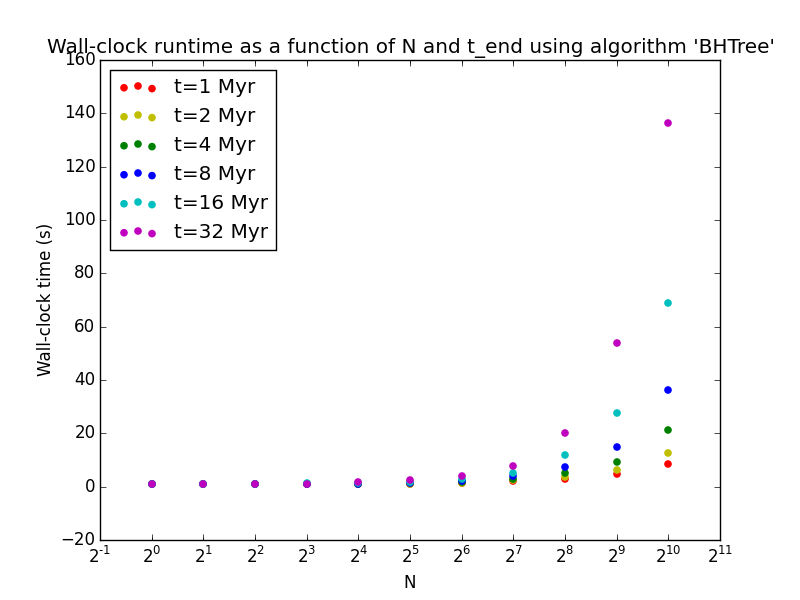
\includegraphics[width=\hsize]{../GravitationalDynamics/plots/CA_GD_TLRH_s1603221_SS_s1617451_BHTree_runtime.png}
      \caption{Wall-clock time as a function of both N and integration 
               end time for BHTree.
              }
         \label{fig:BHTree_runtime}
   \end{figure}
   
   \begin{figure}
   \centering
   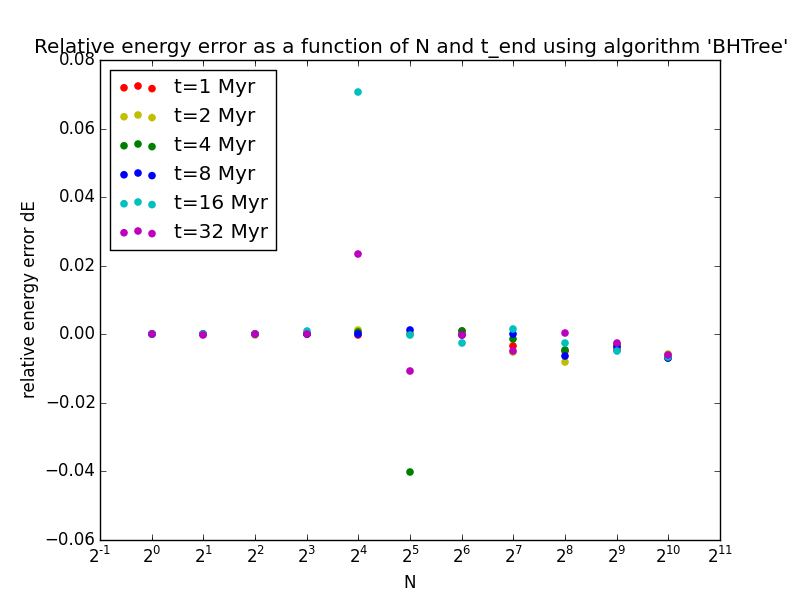
\includegraphics[width=\hsize]{../GravitationalDynamics/plots/CA_GD_TLRH_s1603221_SS_s1617451_BHTree_dE.png}
      \caption{Relative energy error as a function of both N and integration 
               end time for BHTree.
              }
         \label{fig:BHTree_dE}
   \end{figure}

The cluster size $r$ is passed to the nbody\_integrator function as parameter
named `rcl'. This parameter is only used in amuse.units.nbbody\_system, which is
responsible for the creation of bodies within a convined cluster with half-mass
radius `rcl'. The distance between individual particles could increase  as the
cluster half mass radius increases. This maximum distance between particles
scales linearly with the cluster half mass radius. The distance between
particles can be found in the force, but the number of times the force is
calculated does not depend on it. If the cluster size increases and the number
of paricles is unchanged, then at a certain point in time more particles could
be further away. In that case more particles will be bundles together in the
same BHTree, thus, in principle the calculation time could decrease as the
cluster size r increases if particles move further away. 

%__________________________________________________________________

\section{Hermite Algorithm}
   In this section the Hermite algorithm \citep{1995ApJ...443L..93H} will
   be briefly reviewed. The resulting stability criteria will be
   rewritten in terms of local state variables, local timescales and
   constitutive relations.
   
   Figure~\ref{fig:Hermite_runtime} and Figure~\ref{fig:Hermite_dE}


   \begin{figure}
   \centering
   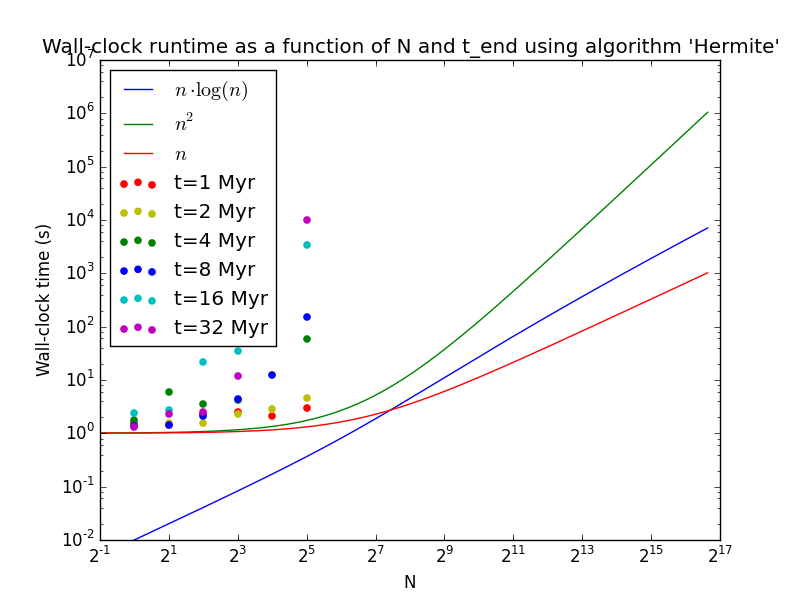
\includegraphics[width=\hsize]{../GravitationalDynamics/plots/CA_GD_TLRH_s1603221_SS_s1617451_Hermite_runtime.png}
      \caption{Wall-clock time as a function of both N and integration 
               end time for Hermite.
              }
         \label{fig:Hermite_runtime}
   \end{figure}
   
   \begin{figure}
   \centering
   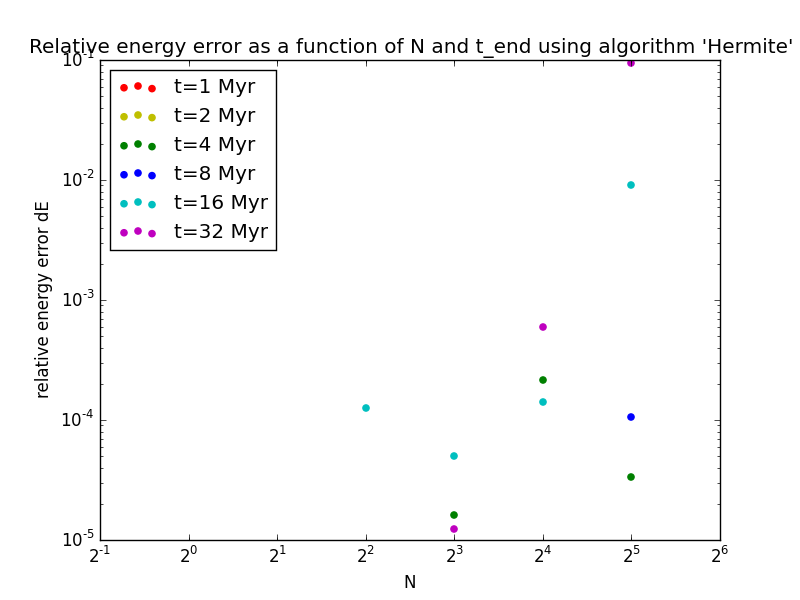
\includegraphics[width=\hsize]{../GravitationalDynamics/plots/CA_GD_TLRH_s1603221_SS_s1617451_Hermite_dE.png}
      \caption{Relative energy error as a function of both N and integration 
               end time for Hermite.
              }
         \label{fig:Hermite_dE}
   \end{figure}

\section{Huayno Algorithm}
  \citep{2012NewA...17..711P}
  
   \begin{figure}
   \centering
   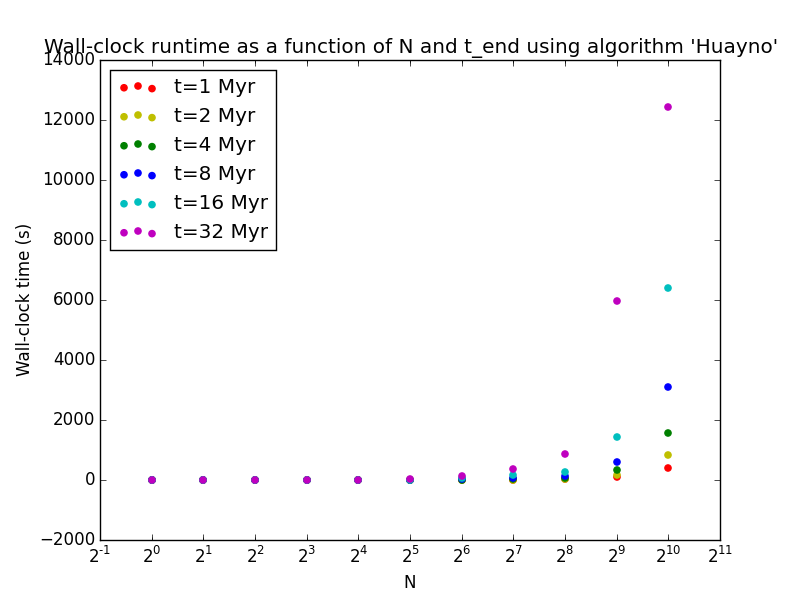
\includegraphics[width=\hsize]{../GravitationalDynamics/plots/CA_GD_TLRH_s1603221_SS_s1617451_Huayno_runtime.png}
      \caption{Wall-clock time as a function of both N and integration 
               end time for Huayno.
              }
         \label{fig:Huayno_runtime}
   \end{figure}
   
   \begin{figure}
   \centering
   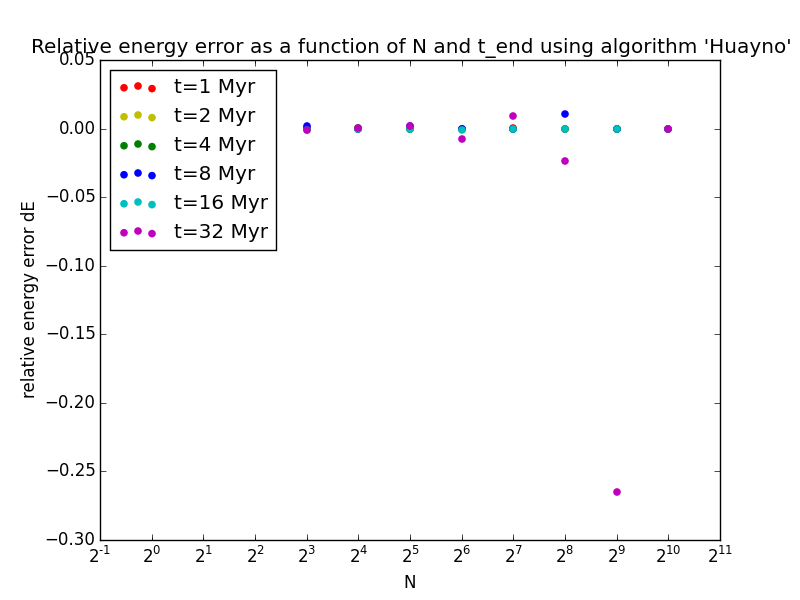
\includegraphics[width=\hsize]{../GravitationalDynamics/plots/CA_GD_TLRH_s1603221_SS_s1617451_Huayno_dE.png}
      \caption{Relative energy error as a function of both N and integration 
               end time for Huayno.
              }
         \label{fig:Huayno_dE}
   \end{figure}


\section{Bound Cluster Mass}
  In this section we discuss two different methods used to determine whether
  a star is bound or unbound by the gravitational forces of the other stars in the 
  galaxy working on it. Moreover, we discuss the differences between both
  algorithms and we conclude that the built-in is better suited for our needs.
  
  On one hand, AMUSE has a built-in method \citep{1998ApJ...498..137E}
  
  On the other hand, we have written our own routine to calculate the bound mass.
  A vital assumption is that when the kinetic energy $E_k$ of a star is greater than the potential
  energy $E_pot$, the star is unbound. Conversely, the star is unbound.


%%                                     Two column figure (place early!)
%%______________________________________________ Gamma_1 (lg rho, lg e)
%   \begin{figure*}
%   \centering
%   %%%\includegraphics{empty.eps}
%   %%%\includegraphics{empty.eps}
%   %%%\includegraphics{empty.eps}
%   \caption{Adiabatic exponent $\Gamma_1$.
%               $\Gamma_1$ is plotted as a function of
%               $\lg$ internal energy $\mathrm{[erg\,g^{-1}]}$ and $\lg$
%               density $\mathrm{[g\,cm^{-3}]}$.}
%              \label{FigGam}%
%    \end{figure*}
%%

%   Baker (\cite{baker}) investigates the stability of thin layers in
%   self-gravitating,
%   spherical gas clouds with the following properties:
%   \begin{itemize}
%      \item hydrostatic equilibrium,
%      \item thermal equilibrium,
%      \item energy transport by grey radiation diffusion.
%   \end{itemize}
%   For the one-zone-model Baker obtains necessary conditions
%   for dynamical, secular and vibrational (or pulsational)
%   stability (Eqs.\ (34a,\,b,\,c) in Baker \cite{baker}). Using Baker's
%   notation:
%   \[
%      \begin{array}{lp{0.8\linewidth}}
%         M_{r}  & mass internal to the radius $r$     \\
%         m               & mass of the zone                    \\
%         r_0             & unperturbed zone radius             \\
%         \rho_0          & unperturbed density in the zone     \\
%         T_0             & unperturbed temperature in the zone \\
%         L_{r0}          & unperturbed luminosity              \\
%         E_{\mathrm{th}} & thermal energy of the zone
%      \end{array}
%   \]
%\noindent
%   and with the definitions of the \emph{local cooling time\/}
%   (see Fig.~\ref{FigGam})
%   \begin{equation}
%      \tau_{\mathrm{co}} = \frac{E_{\mathrm{th}}}{L_{r0}} \,,
%   \end{equation}
%   and the \emph{local free-fall time}
%   \begin{equation}
%      \tau_{\mathrm{ff}} =
%         \sqrt{ \frac{3 \pi}{32 G} \frac{4\pi r_0^3}{3 M_{\mathrm{r}}}
%}\,,
%   \end{equation}
%   Baker's $K$ and $\sigma_0$ have the following form:
%   \begin{eqnarray}
%      \sigma_0 & = & \frac{\pi}{\sqrt{8}}
%                     \frac{1}{ \tau_{\mathrm{ff}}} \\
%      K        & = & \frac{\sqrt{32}}{\pi} \frac{1}{\delta}
%                        \frac{ \tau_{\mathrm{ff}} }
%                             { \tau_{\mathrm{co}} }\,;
%   \end{eqnarray}
%   where $ E_{\mathrm{th}} \approx m (P_0/{\rho_0})$ has been used and
%   \begin{equation}
%   \begin{array}{l}
%      \delta = - \left(
%                    \frac{ \partial \ln \rho }{ \partial \ln T }
%                 \right)_P \\
%      e=mc^2
%   \end{array}
%   \end{equation}
%   is a thermodynamical quantity which is of order $1$ and equal to $1$
%   for nonreacting mixtures of classical perfect gases. The physical
%   meaning of $ \sigma_0 $ and $K$ is clearly visible in the equations
%   above. $\sigma_0$ represents a frequency of the order one per
%   free-fall time. $K$ is proportional to the ratio of the free-fall
%   time and the cooling time. Substituting into Baker's criteria, using
%   thermodynamic identities and definitions of thermodynamic quantities,
%   \begin{displaymath}
%      \Gamma_1      = \left( \frac{ \partial \ln P}{ \partial\ln \rho}
%                           \right)_{S}    \, , \;
%      \chi^{}_\rho  = \left( \frac{ \partial \ln P}{ \partial\ln \rho}
%                           \right)_{T}    \, , \;
%      \kappa^{}_{P} = \left( \frac{ \partial \ln \kappa}{ \partial\ln P}
%                           \right)_{T}
%   \end{displaymath}
%   \begin{displaymath}
%      \nabla_{\mathrm{ad}} = \left( \frac{ \partial \ln T}
%                             { \partial\ln P} \right)_{S} \, , \;
%      \chi^{}_T       = \left( \frac{ \partial \ln P}
%                             { \partial\ln T} \right)_{\rho} \, , \;
%      \kappa^{}_{T}   = \left( \frac{ \partial \ln \kappa}
%                             { \partial\ln T} \right)_{T}
%   \end{displaymath}
%   one obtains, after some pages of algebra, the conditions for
%   \emph{stability\/} given
%   below:
%   \begin{eqnarray}
%      \frac{\pi^2}{8} \frac{1}{\tau_{\mathrm{ff}}^2}
%                ( 3 \Gamma_1 - 4 )
%         & > & 0 \label{ZSDynSta} \\
%      \frac{\pi^2}{\tau_{\mathrm{co}}
%                   \tau_{\mathrm{ff}}^2}
%                   \Gamma_1 \nabla_{\mathrm{ad}}
%                   \left[ \frac{ 1- 3/4 \chi^{}_\rho }{ \chi^{}_T }
%                          ( \kappa^{}_T - 4 )
%                        + \kappa^{}_P + 1
%                   \right]
%        & > & 0 \label{ZSSecSta} \\
%     \frac{\pi^2}{4} \frac{3}{\tau_{ \mathrm{co} }
%                              \tau_{ \mathrm{ff} }^2
%                             }
%         \Gamma_1^2 \, \nabla_{\mathrm{ad}} \left[
%                                   4 \nabla_{\mathrm{ad}}
%                                   - ( \nabla_{\mathrm{ad}} \kappa^{}_T
%                                     + \kappa^{}_P
%                                     )
%                                   - \frac{4}{3 \Gamma_1}
%                                \right]
%        & > & 0   \label{ZSVibSta}
%   \end{eqnarray}
%%
%   For a physical discussion of the stability criteria see Baker
%   (\cite{baker}) or Cox (\cite{cox}).
%
%   We observe that these criteria for dynamical, secular and
%   vibrational stability, respectively, can be factorized into
%   \begin{enumerate}
%      \item a factor containing local timescales only,
%      \item a factor containing only constitutive relations and
%         their derivatives.
%   \end{enumerate}
%   The first factors, depending on only timescales, are positive
%   by definition. The signs of the left hand sides of the
%   inequalities~(\ref{ZSDynSta}), (\ref{ZSSecSta}) and (\ref{ZSVibSta})
%   therefore depend exclusively on the second factors containing
%   the constitutive relations. Since they depend only
%   on state variables, the stability criteria themselves are \emph{
%   functions of the thermodynamic state in the local zone}. The
%   one-zone stability can therefore be determined
%   from a simple equation of state, given for example, as a function
%   of density and
%   temperature. Once the microphysics, i.e.\ the thermodynamics
%   and opacities (see Table~\ref{KapSou}), are specified (in practice
%   by specifying a chemical composition) the one-zone stability can
%   be inferred if the thermodynamic state is specified.
%   The zone -- or in
%   other words the layer -- will be stable or unstable in
%   whatever object it is imbedded as long as it satisfies the
%   one-zone-model assumptions. Only the specific growth rates
%   (depending upon the time scales) will be different for layers
%   in different objects.

%%__________________________________________________ One column table
%   \begin{table}
%      \caption[]{Opacity sources.}
%         \label{KapSou}
%     $$ 
%         \begin{array}{p{0.5\linewidth}l}
%            \hline
%            \noalign{\smallskip}
%            Source      &  T / {[\mathrm{K}]} \\
%            \noalign{\smallskip}
%            \hline
%            \noalign{\smallskip}
%            Yorke 1979, Yorke 1980a & \leq 1700^{\mathrm{a}}     \\
%%           Yorke 1979, Yorke 1980a & \leq 1700             \\
%            Kr\"ugel 1971           & 1700 \leq T \leq 5000 \\
%            Cox \& Stewart 1969     & 5000 \leq             \\
%            \noalign{\smallskip}
%            \hline
%         \end{array}
%     $$ 
%   \end{table}
%%
%   We will now write down the sign (and therefore stability)
%   determining parts of the left-hand sides of the inequalities
%   (\ref{ZSDynSta}), (\ref{ZSSecSta}) and (\ref{ZSVibSta}) and thereby
%   obtain \emph{stability equations of state}.
%
%   The sign determining part of inequality~(\ref{ZSDynSta}) is
%   $3\Gamma_1 - 4$ and it reduces to the
%   criterion for dynamical stability
%   \begin{equation}
%     \Gamma_1 > \frac{4}{3}\,\cdot
%   \end{equation}
%   Stability of the thermodynamical equilibrium demands
%   \begin{equation}
%      \chi^{}_\rho > 0, \;\;  c_v > 0\, ,
%   \end{equation}
%   and
%   \begin{equation}
%      \chi^{}_T > 0
%   \end{equation}
%   holds for a wide range of physical situations.
%   With
%   \begin{eqnarray}
%      \Gamma_3 - 1 = \frac{P}{\rho T} \frac{\chi^{}_T}{c_v}&>&0\\
%      \Gamma_1     = \chi_\rho^{} + \chi_T^{} (\Gamma_3 -1)&>&0\\
%      \nabla_{\mathrm{ad}}  = \frac{\Gamma_3 - 1}{\Gamma_1}         &>&0
%   \end{eqnarray}
%   we find the sign determining terms in inequalities~(\ref{ZSSecSta})
%   and (\ref{ZSVibSta}) respectively and obtain the following form
%   of the criteria for dynamical, secular and vibrational
%   \emph{stability}, respectively:
%   \begin{eqnarray}
%      3 \Gamma_1 - 4 =: S_{\mathrm{dyn}}      > & 0 & \label{DynSta}  \\
%%
%      \frac{ 1- 3/4 \chi^{}_\rho }{ \chi^{}_T } ( \kappa^{}_T - 4 )
%         + \kappa^{}_P + 1 =: S_{\mathrm{sec}} > & 0 & \label{SecSta} \\
%%
%      4 \nabla_{\mathrm{ad}} - (\nabla_{\mathrm{ad}} \kappa^{}_T
%                             + \kappa^{}_P)
%                             - \frac{4}{3 \Gamma_1} =: S_{\mathrm{vib}}
%                                      > & 0\,.& \label{VibSta}
%   \end{eqnarray}
%   The constitutive relations are to be evaluated for the
%   unperturbed thermodynamic state (say $(\rho_0, T_0)$) of the zone.
%   We see that the one-zone stability of the layer depends only on
%   the constitutive relations $\Gamma_1$,
%   $\nabla_{\mathrm{ad}}$, $\chi_T^{},\,\chi_\rho^{}$,
%   $\kappa_P^{},\,\kappa_T^{}$.
%   These depend only on the unperturbed
%   thermodynamical state of the layer. Therefore the above relations
%   define the one-zone-stability equations of state
%   $S_{\mathrm{dyn}},\,S_{\mathrm{sec}}$
%   and $S_{\mathrm{vib}}$. See Fig.~\ref{FigVibStab} for a picture of
%   $S_{\mathrm{vib}}$. Regions of secular instability are
%   listed in Table~1.
%
%%
%%                                                One column figure
%%----------------------------------------------------------- S_vib
%   \begin{figure}
%   \centering
%   %%%\includegraphics[width=3cm]{empty.eps}
%      \caption{Vibrational stability equation of state
%               $S_{\mathrm{vib}}(\lg e, \lg \rho)$.
%               $>0$ means vibrational stability.
%              }
%         \label{FigVibStab}
%   \end{figure}
%%
%%______________________________________________________________
%


\section{Conclusions}

   \begin{enumerate}
      \item Conlcusie 1
      \item Conclusie 2
      \item Conclusie 3
   \end{enumerate}

\begin{acknowledgements}
      The authors are grateful for the help of their supervisors
      Edwin van der Helm, MSc and Prof.dr. S.F. Portegies Zwart.
\end{acknowledgements}


%-------------------------------------------------------------------

\bibliographystyle{aa} 
%\setlength{\bibsep}{0pt} % Remove whitespace in bibliography.
\bibliography{CA_GD_TLRH_s1603221_SS_s1617451_report} 

%\begin{thebibliography}{}
%
%  \bibitem[1966]{baker} Baker, N. 1966,
%      in Stellar Evolution,
%      ed.\ R. F. Stein,\& A. G. W. Cameron
%      (Plenum, New York) 333
%
%   \bibitem[1988]{balluch} Balluch, M. 1988,
%      A\&A, 200, 58
%
%   \bibitem[1980]{cox} Cox, J. P. 1980,
%      Theory of Stellar Pulsation
%      (Princeton University Press, Princeton) 165
%
%   \bibitem[1969]{cox69} Cox, A. N.,\& Stewart, J. N. 1969,
%      Academia Nauk, Scientific Information 15, 1
%
%   \bibitem[1980]{mizuno} Mizuno H. 1980,
%      Prog. Theor. Phys., 64, 544
%   
%   \bibitem[1987]{tscharnuter} Tscharnuter W. M. 1987,
%      A\&A, 188, 55
%  
%   \bibitem[1992]{terlevich} Terlevich, R. 1992, in ASP Conf. Ser. 31, 
%      Relationships between Active Galactic Nuclei and Starburst Galaxies, 
%      ed. A. V. Filippenko, 13
%
%   \bibitem[1980a]{yorke80a} Yorke, H. W. 1980a,
%      A\&A, 86, 286
%
%   \bibitem[1997]{zheng} Zheng, W., Davidsen, A. F., Tytler, D. \& Kriss, G. A.
%      1997, preprint
%\end{thebibliography}

\end{document}

%%%%%%%%%%%%%%%%%%%%%%%%%%%%%%%%%%%%%%%%%%%%%%%%%%%%%%%%%%%%%%
Examples for figures using graphicx
A guide "Using Imported Graphics in LaTeX2e"  (Keith Reckdahl)
is available on a lot of LaTeX public servers or ctan mirrors.
The file is : epslatex.pdf 
%%%%%%%%%%%%%%%%%%%%%%%%%%%%%%%%%%%%%%%%%%%%%%%%%%%%%%%%%%%%%%

%_____________________________________________________________
%                 A figure as large as the width of the column
%-------------------------------------------------------------
   \begin{figure}
   \centering
   \includegraphics[width=\hsize]{empty.eps}
      \caption{Vibrational stability equation of state
               $S_{\mathrm{vib}}(\lg e, \lg \rho)$.
               $>0$ means vibrational stability.
              }
         \label{FigVibStab}
   \end{figure}
%
%_____________________________________________________________
%                                    One column rotated figure
%-------------------------------------------------------------
   \begin{figure}
   \centering
   \includegraphics[angle=-90,width=3cm]{empty.eps}
      \caption{Vibrational stability equation of state
               $S_{\mathrm{vib}}(\lg e, \lg \rho)$.
               $>0$ means vibrational stability.
              }
         \label{FigVibStab}
   \end{figure}
%
%_____________________________________________________________
%                        Figure with caption on the right side 
%-------------------------------------------------------------
   \begin{figure}
   \sidecaption
   \includegraphics[width=3cm]{empty.eps}
      \caption{Vibrational stability equation of state
               $S_{\mathrm{vib}}(\lg e, \lg \rho)$.
               $>0$ means vibrational stability.
              }
         \label{FigVibStab}
   \end{figure}
%
%_____________________________________________________________
%
%_____________________________________________________________
%                                Figure with a new BoundingBox 
%-------------------------------------------------------------
   \begin{figure}
   \centering
   \includegraphics[bb=10 20 100 300,width=3cm,clip]{empty.eps}
      \caption{Vibrational stability equation of state
               $S_{\mathrm{vib}}(\lg e, \lg \rho)$.
               $>0$ means vibrational stability.
              }
         \label{FigVibStab}
   \end{figure}
%
%_____________________________________________________________
%
%_____________________________________________________________
%                                      The "resizebox" command 
%-------------------------------------------------------------
   \begin{figure}
   \resizebox{\hsize}{!}
            {\includegraphics[bb=10 20 100 300,clip]{empty.eps}
      \caption{Vibrational stability equation of state
               $S_{\mathrm{vib}}(\lg e, \lg \rho)$.
               $>0$ means vibrational stability.
              }
         \label{FigVibStab}
   \end{figure}
%
%______________________________________________________________
%
%_____________________________________________________________
%                                             Two column Figure 
%-------------------------------------------------------------
   \begin{figure*}
   \resizebox{\hsize}{!}
            {\includegraphics[bb=10 20 100 300,clip]{empty.eps}
      \caption{Vibrational stability equation of state
               $S_{\mathrm{vib}}(\lg e, \lg \rho)$.
               $>0$ means vibrational stability.
              }
         \label{FigVibStab}
   \end{figure*}
%
%______________________________________________________________
%
%_____________________________________________________________
%                                             Simple A&A Table
%_____________________________________________________________
%
\begin{table}
\caption{Nonlinear Model Results}             % title of Table
\label{table:1}      % is used to refer this table in the text
\centering                          % used for centering table
\begin{tabular}{c c c c}        % centered columns (4 columns)
\hline\hline                 % inserts double horizontal lines
HJD & $E$ & Method\#2 & Method\#3 \\    % table heading 
\hline                        % inserts single horizontal line
   1 & 50 & $-837$ & 970 \\      % inserting body of the table
   2 & 47 & 877    & 230 \\
   3 & 31 & 25     & 415 \\
   4 & 35 & 144    & 2356 \\
   5 & 45 & 300    & 556 \\ 
\hline                                   %inserts single line
\end{tabular}
\end{table}
%
%_____________________________________________________________
%                                             Two column Table 
%_____________________________________________________________
%
\begin{table*}
\caption{Nonlinear Model Results}             
\label{table:1}      
\centering          
\begin{tabular}{c c c c l l l }     % 7 columns 
\hline\hline       
                      % To combine 4 columns into a single one 
HJD & $E$ & Method\#2 & \multicolumn{4}{c}{Method\#3}\\ 
\hline                    
   1 & 50 & $-837$ & 970 & 65 & 67 & 78\\  
   2 & 47 & 877    & 230 & 567& 55 & 78\\
   3 & 31 & 25     & 415 & 567& 55 & 78\\
   4 & 35 & 144    & 2356& 567& 55 & 78 \\
   5 & 45 & 300    & 556 & 567& 55 & 78\\
\hline                  
\end{tabular}
\end{table*}
%
%-------------------------------------------------------------
%                                          Table with notes 
%-------------------------------------------------------------
%
% A single note
\begin{table}
\caption{\label{t7}Spectral types and photometry for stars in the
  region.}
\centering
\begin{tabular}{lccc}
\hline\hline
Star&Spectral type&RA(J2000)&Dec(J2000)\\
\hline
69           &B1\,V     &09 15 54.046 & $-$50 00 26.67\\
49           &B0.7\,V   &*09 15 54.570& $-$50 00 03.90\\
LS~1267~(86) &O8\,V     &09 15 52.787&11.07\\
24.6         &7.58      &1.37 &0.20\\
\hline
LS~1262      &B0\,V     &09 15 05.17&11.17\\
MO 2-119     &B0.5\,V   &09 15 33.7 &11.74\\
LS~1269      &O8.5\,V   &09 15 56.60&10.85\\
\hline
\end{tabular}
\tablefoot{The top panel shows likely members of Pismis~11. The second
panel contains likely members of Alicante~5. The bottom panel
displays stars outside the clusters.}
\end{table}
%
% More notes
%
\begin{table}
\caption{\label{t7}Spectral types and photometry for stars in the
  region.}
\centering
\begin{tabular}{lccc}
\hline\hline
Star&Spectral type&RA(J2000)&Dec(J2000)\\
\hline
69           &B1\,V     &09 15 54.046 & $-$50 00 26.67\\
49           &B0.7\,V   &*09 15 54.570& $-$50 00 03.90\\
LS~1267~(86) &O8\,V     &09 15 52.787&11.07\tablefootmark{a}\\
24.6         &7.58\tablefootmark{1}&1.37\tablefootmark{a}   &0.20\tablefootmark{a}\\
\hline
LS~1262      &B0\,V     &09 15 05.17&11.17\tablefootmark{b}\\
MO 2-119     &B0.5\,V   &09 15 33.7 &11.74\tablefootmark{c}\\
LS~1269      &O8.5\,V   &09 15 56.60&10.85\tablefootmark{d}\\
\hline
\end{tabular}
\tablefoot{The top panel shows likely members of Pismis~11. The second
panel contains likely members of Alicante~5. The bottom panel
displays stars outside the clusters.\\
\tablefoottext{a}{Photometry for MF13, LS~1267 and HD~80077 from
Dupont et al.}
\tablefoottext{b}{Photometry for LS~1262, LS~1269 from
Durand et al.}
\tablefoottext{c}{Photometry for MO2-119 from
Mathieu et al.}
}
\end{table}
%
%-------------------------------------------------------------
%                                       Table with references 
%-------------------------------------------------------------
%
\begin{table*}[h]
 \caption[]{\label{nearbylistaa2}List of nearby SNe used in this work.}
\begin{tabular}{lccc}
 \hline \hline
  SN name &
  Epoch &
 Bands &
  References \\
 &
  (with respect to $B$ maximum) &
 &
 \\ \hline
1981B   & 0 & {\it UBV} & 1\\
1986G   &  $-$3, $-$1, 0, 1, 2 & {\it BV}  & 2\\
1989B   & $-$5, $-$1, 0, 3, 5 & {\it UBVRI}  & 3, 4\\
1990N   & 2, 7 & {\it UBVRI}  & 5\\
1991M   & 3 & {\it VRI}  & 6\\
\hline
\noalign{\smallskip}
\multicolumn{4}{c}{ SNe 91bg-like} \\
\noalign{\smallskip}
\hline
1991bg   & 1, 2 & {\it BVRI}  & 7\\
1999by   & $-$5, $-$4, $-$3, 3, 4, 5 & {\it UBVRI}  & 8\\
\hline
\noalign{\smallskip}
\multicolumn{4}{c}{ SNe 91T-like} \\
\noalign{\smallskip}
\hline
1991T   & $-$3, 0 & {\it UBVRI}  &  9, 10\\
2000cx  & $-$3, $-$2, 0, 1, 5 & {\it UBVRI}  & 11\\ %
\hline
\end{tabular}
\tablebib{(1)~\citet{branch83};
(2) \citet{phillips87}; (3) \citet{barbon90}; (4) \citet{wells94};
(5) \citet{mazzali93}; (6) \citet{gomez98}; (7) \citet{kirshner93};
(8) \citet{patat96}; (9) \citet{salvo01}; (10) \citet{branch03};
(11) \citet{jha99}.
}
\end{table}
%_____________________________________________________________
%                      A rotated Two column Table in landscape  
%-------------------------------------------------------------
\begin{sidewaystable*}
\caption{Summary for ISOCAM sources with mid-IR excess 
(YSO candidates).}\label{YSOtable}
\centering
\begin{tabular}{crrlcl} 
\hline\hline             
ISO-L1551 & $F_{6.7}$~[mJy] & $\alpha_{6.7-14.3}$ 
& YSO type$^{d}$ & Status & Comments\\
\hline
  \multicolumn{6}{c}{\it New YSO candidates}\\ % To combine 6 columns into a single one
\hline
  1 & 1.56 $\pm$ 0.47 & --    & Class II$^{c}$ & New & Mid\\
  2 & 0.79:           & 0.97: & Class II ?     & New & \\
  3 & 4.95 $\pm$ 0.68 & 3.18  & Class II / III & New & \\
  5 & 1.44 $\pm$ 0.33 & 1.88  & Class II       & New & \\
\hline
  \multicolumn{6}{c}{\it Previously known YSOs} \\
\hline
  61 & 0.89 $\pm$ 0.58 & 1.77 & Class I & \object{HH 30} & Circumstellar disk\\
  96 & 38.34 $\pm$ 0.71 & 37.5& Class II& MHO 5          & Spectral type\\
\hline
\end{tabular}
\end{sidewaystable*}
%_____________________________________________________________
%                      A rotated One column Table in landscape  
%-------------------------------------------------------------
\begin{sidewaystable}
\caption{Summary for ISOCAM sources with mid-IR excess 
(YSO candidates).}\label{YSOtable}
\centering
\begin{tabular}{crrlcl} 
\hline\hline             
ISO-L1551 & $F_{6.7}$~[mJy] & $\alpha_{6.7-14.3}$ 
& YSO type$^{d}$ & Status & Comments\\
\hline
  \multicolumn{6}{c}{\it New YSO candidates}\\ % To combine 6 columns into a single one
\hline
  1 & 1.56 $\pm$ 0.47 & --    & Class II$^{c}$ & New & Mid\\
  2 & 0.79:           & 0.97: & Class II ?     & New & \\
  3 & 4.95 $\pm$ 0.68 & 3.18  & Class II / III & New & \\
  5 & 1.44 $\pm$ 0.33 & 1.88  & Class II       & New & \\
\hline
  \multicolumn{6}{c}{\it Previously known YSOs} \\
\hline
  61 & 0.89 $\pm$ 0.58 & 1.77 & Class I & \object{HH 30} & Circumstellar disk\\
  96 & 38.34 $\pm$ 0.71 & 37.5& Class II& MHO 5          & Spectral type\\
\hline
\end{tabular}
\end{sidewaystable}
%
%_____________________________________________________________
%                              Table longer than a single page  
%-------------------------------------------------------------
% All long tables will be placed automatically at the end, after 
%                                        \end{thebibliography}
%
\begin{longtab}
\begin{longtable}{lllrrr}
\caption{\label{kstars} Sample stars with absolute magnitude}\\
\hline\hline
Catalogue& $M_{V}$ & Spectral & Distance & Mode & Count Rate \\
\hline
\endfirsthead
\caption{continued.}\\
\hline\hline
Catalogue& $M_{V}$ & Spectral & Distance & Mode & Count Rate \\
\hline
\endhead
\hline
\endfoot
%%
Gl 33    & 6.37 & K2 V & 7.46 & S & 0.043170\\
Gl 66AB  & 6.26 & K2 V & 8.15 & S & 0.260478\\
Gl 68    & 5.87 & K1 V & 7.47 & P & 0.026610\\
         &      &      &      & H & 0.008686\\
Gl 86 
\footnote{Source not included in the HRI catalog. See Sect.~5.4.2 for details.}
         & 5.92 & K0 V & 10.91& S & 0.058230\\
\end{longtable}
\end{longtab}
%
%_____________________________________________________________
%                              Table longer than a single page
%                                             and in landscape 
%  In the preamble, use:       \usepackage{lscape}
%-------------------------------------------------------------
% All long tables will be placed automatically at the end, after
%                                        \end{thebibliography}
%
\begin{longtab}
\begin{landscape}
\begin{longtable}{lllrrr}
\caption{\label{kstars} Sample stars with absolute magnitude}\\
\hline\hline
Catalogue& $M_{V}$ & Spectral & Distance & Mode & Count Rate \\
\hline
\endfirsthead
\caption{continued.}\\
\hline\hline
Catalogue& $M_{V}$ & Spectral & Distance & Mode & Count Rate \\
\hline
\endhead
\hline
\endfoot
%%
Gl 33    & 6.37 & K2 V & 7.46 & S & 0.043170\\
Gl 66AB  & 6.26 & K2 V & 8.15 & S & 0.260478\\
Gl 68    & 5.87 & K1 V & 7.47 & P & 0.026610\\
         &      &      &      & H & 0.008686\\
Gl 86
\footnote{Source not included in the HRI catalog. See Sect.~5.4.2 for details.}
         & 5.92 & K0 V & 10.91& S & 0.058230\\
\end{longtable}
\end{landscape}
\end{longtab}
%
% Online Material
%_____________________________________________________________
%        Online appendices have to be placed at the end, after
%                                        \end{thebibliography}
%-------------------------------------------------------------
\end{thebibliography}

\Online

\begin{appendix} %First online appendix
\section{Background galaxy number counts and shear noise-levels}
Because the optical images used in this analysis...

\begin{figure*}
\centering
\includegraphics[width=16.4cm,clip]{1787f24.ps}
\caption{Plotted above...}
\label{appfig}
\end{figure*}

Because the optical images...
\end{appendix}

\begin{appendix} %Second online appendix
These studies, however, have faced...
\end{appendix}

\end{document}
%
%_____________________________________________________________
%        Some tables or figures are in the printed version and
%                      some are only in the electronic version
%-------------------------------------------------------------
%
% Leave all the tables or figures in the text, at their right place 
% and use the commands \onlfig{} and \onltab{}. These elements
% will be automatically placed at the end, in the section
% Online material.

\documentclass{aa}
...
\begin{document}
text of the paper...
\begin{figure*}%f1
\includegraphics[width=10.9cm]{1787f01.eps}
\caption{Shown in greyscale is a...}
\label{cl12301}}
\end{figure*}
...
from the intrinsic ellipticity distribution.
% Figure 2 available electronically only
\onlfig{
\begin{figure*}%f2
\includegraphics[width=11.6cm]{1787f02.eps}
\caption {Shown in greyscale...}
\label{cl1018}
\end{figure*}
}

% Figure 3 available electronically only
\onlfig{
\begin{figure*}%f3
\includegraphics[width=11.2cm]{1787f03.eps}
\caption{Shown in panels...}
\label{cl1059}
\end{figure*}
}

\begin{figure*}%f4
\includegraphics[width=10.9cm]{1787f04.eps}
\caption{Shown in greyscale is...}
\label{cl1232}}
\end{figure*}

\begin{table}%t1
\caption{Complexes characterisation.}\label{starbursts}
\centering
\begin{tabular}{lccc}
\hline \hline
Complex & $F_{60}$ & 8.6 &  No. of  \\
...
\hline
\end{tabular}
\end{table}
The second method produces...

% Figure 5 available electronically only
\onlfig{
\begin{figure*}%f5
\includegraphics[width=11.2cm]{1787f05.eps}
\caption{Shown in panels...}
\label{cl1238}}
\end{figure*}
}

As can be seen, in general the deeper...
% Table 2 available electronically only
\onltab{
\begin{table*}%t2
\caption{List of the LMC stellar complexes...}\label{Properties}
\centering
\begin{tabular}{lccccccccc}
\hline  \hline
Stellar & RA & Dec & ...
...
\hline
\end{tabular}
\end{table*}
}

% Table 3 available electronically only
\onltab{
\begin{table*}%t3
\caption{List of the derived...}\label{IrasFluxes}
\centering
\begin{tabular}{lcccccccccc}
\hline \hline
Stellar & $f12$ & $L12$ &...
...
\hline
\end{tabular}
\end{table*}
}
%
%-------------------------------------------------------------
%     For the online material, table longer than a single page
%                 In the preamble for landscape case, use : 
%                                          \usepackage{lscape}
%-------------------------------------------------------------
\documentclass{aa}
\usepackage[varg]{txfonts}
\usepackage{graphicx}
\usepackage{lscape}

\begin{document}
text of the paper
% Table will be print automatically at the end, in the section Online material.
\onllongtab{
\begin{longtable}{lrcrrrrrrrrl}
\caption{Line data and abundances ...}\\
\hline
\hline
Def & mol & Ion & $\lambda$ & $\chi$ & $\log gf$ & N & e &  rad & $\delta$ & $\delta$ 
red & References \\
\hline
\endfirsthead
\caption{Continued.} \\
\hline
Def & mol & Ion & $\lambda$ & $\chi$ & $\log gf$ & B & C &  rad & $\delta$ & $\delta$ 
red & References \\
\hline
\endhead
\hline
\endfoot
\hline
\endlastfoot
A & CH & 1 &3638 & 0.002 & $-$2.551 &  &  &  & $-$150 & 150 &  Jorgensen et al. (1996) \\                    
\end{longtable}
}% End onllongtab

% Or for landscape, large table:

\onllongtab{
\begin{landscape}
\begin{longtable}{lrcrrrrrrrrl}
...
\end{longtable}
\end{landscape}
}% End onllongtab
